The SZ-effect, or {\it SZE}, in clusters is a spectral distortion of
the CMB radiation due to inverse Compton scattering of the relatively
cool CMB photons off hot ICM electrons.  At frequencies less than 218
GHz, the intensity of the CMB radiation is diminished compared to the
unscattered CMB, and the SZ effect is manifested as a brightness
temperature decrement towards the cluster. This decrement, $\Delta
T_{\it SZ}/T_{\it CMB}$, has a magnitude proportional to the Compton
$y$-parameter, i.e., the total number of scatterers (electrons)
weighted by their associated temperature:

\begin{equation}
y = \integral{\infty}{-\infty}{n_e {{k_B T_e}\over{m_e c^2}}\sigma_T}{\ell},
\end{equation}

where I treat the cluster as effectively infinitely far away and
define $\ell = 0$ to be at the cluster center.  This equation holds
for any line of sight through the cluster.  What we measure in SZ
observations is the projected 2D image of the cluster, where the value
at each location $\theta$ is given by this line integral, or

\begin{equation}
y(\theta) = {{\sigma_T}\over{m_e c^2}}\integral{\infty}{-\infty}{P_e(r(\ell,\theta))}{\ell}
\end{equation}

if we identify $P_e = n_e k_B T_e$.

\begin{figure}[th]
\begin{center}
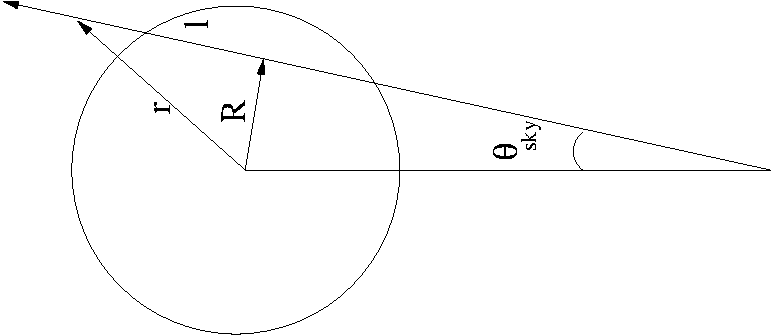
\includegraphics[scale=0.5]{figures/szmodel.jpg}\\
\end{center}
\caption{Schematic of the line integration through a cluster for
  constructing a projected 2D profile from a 3D radially-symmetric model.}
\end{figure}

For each $\theta$ on the sky, there is a cylindrical radius $R_\theta
= D_A\theta$ that corresponds to a physical separation of that line of
sight from the center of the cluster. With $\ell$ defined to be zero
at the cluster center, for an axially-symmetric pressure model
$P(r)$ we have

\begin{eqnarray}
r^2 &=& \ell^2 + R_\theta^2\\
r\,dr &=& \ell\,d\ell\\
d\ell &=& {{r\,dr}\over{\sqrt{r^2 - R_\theta^2}}}
\end{eqnarray}

and 

\begin{equation}
y(\theta) = {{\sigma_T}\over{m_e c^2}}\integral{\infty}{-\infty}{{{P(r)r}\over{\sqrt{r^2 - R_\theta^2}}}}{r}
\end{equation}

In practice we treat $P(r)$ as a shape function $P(r) = P_0\,p(r)$ and
compute the 2D projection of $p(r)$.  Furthermore, we define the model
in terms of $x\equiv r/r_c$, or $dr = r_c\,dx$ yielding:

\begin{eqnarray}
y(\theta) &=& {{\sigma_T}\over{m_e c^2}}P_0r_c\integral{\infty}{-\infty}{{{p(x)x}\over{\sqrt{x^2 - x^2_\theta}}}}{x}\\\nonumber
          &=& {{\sigma_T}\over{m_e c^2}}P_0D_A\theta_c\integral{\infty}{-\infty}{{{p(x)x}\over{\sqrt{x^2 - x^2_\theta}}}}{x}\\\nonumber
\end{eqnarray}

where $x_\theta\equiv R_\theta/r_c$.  Internally, \climax\ actually
computes the unity-normalized version of the integral, $N(\theta)$
i.e.,

\begin{eqnarray}
I(\theta) &=& \integral{\infty}{-\infty}{{{p(x)x}\over{\sqrt{x^2 - x^2_\theta}}}}{x}\\\nonumber
N(\theta) &=& I(\theta)/I(0)
\end{eqnarray}

and fits $y(\theta) = y(0)N(\theta)$, so that

\begin{eqnarray}
y(0)N(\theta) &=& {{\sigma_T}\over{m_e c^2}} P_0D_A\theta_c I(\theta)\\\nonumber
              &\equiv& {{\sigma_T}\over{m_e c^2}} P_0D_A\theta_c I(0)N(\theta)
\end{eqnarray}

This means that for \climax\ fits to radially-symmetric pressure
models, the pressure normalization can be recovered from:

\begin{equation}
P_0 = y(0)\left({{m_e c^2}\over{\sigma_T D_A\theta_c}}\right){1\over{I(0)}}
\label{eq:ytop}
\end{equation}

when models are normalized in Compton-$y$ units.  Note that I
explicitly retain $I(0)$ in the normalization, since the models $P(r)$
are not in general defined to yield $P_0$ at $\theta = 0$.  (The GNFW
model for example (see \ref{sec:gnfw}) is actually singular at $r=0$
and therefore not technically integrable at $\theta = 0$.  And the
Arnaud model is only fit to $r = 0.03\,\R500$, for which $I(\theta)
\sim 0.89$).

Since the proportionality between Compton $y$ and $\dtsz$ is given by:

\begin{equation}
{{\dtsz}\over{\tcmb}} = f(\nu)\,y
\label{eq:ynu}
\end{equation}

where $f(\nu)$ is a function that encapsulates the frequency
dependence of the SZ effect ($f(\nu) \sim -2$ at $\nu = 30$~GHz, see
Eq.~\ref{eq:fnu}) the pressure normalization is given by:

\begin{equation}
P_0 = {{\dtsz(0)}\over{\tcmb f(\nu)}}\left({{m_e c^2}\over{\sigma_T D_A\theta_c}}\right){1\over{I(0)}}
\end{equation}

when models are normalized in temperature units in \climax.

